\let\negmedspace\undefined
\let\negthickspace\undefined
\documentclass[journal]{IEEEtran}
\usepackage[a5paper, margin=10mm, onecolumn]{geometry}
%\usepackage{lmodern} % Ensure lmodern is loaded for pdflatex
\usepackage{tfrupee} % Include tfrupee package

\setlength{\headheight}{1cm} % Set the height of the header box
\setlength{\headsep}{0mm}     % Set the distance between the header box and the top of the text

\usepackage{gvv-book}
\usepackage{gvv}
\usepackage{cite}
\usepackage{amsmath,amssymb,amsfonts,amsthm}
\usepackage{algorithmic}
\usepackage{graphicx}
\usepackage{textcomp}
\usepackage{xcolor}
\usepackage{txfonts}
\usepackage{listings}
\usepackage{enumitem}
\usepackage{mathtools}
\usepackage{gensymb}
\usepackage{comment}
\usepackage[breaklinks=true]{hyperref}
\usepackage{tkz-euclide} 
\usepackage{listings}
% \usepackage{gvv}                                        
\def\inputGnumericTable{}                                 
\usepackage[latin1]{inputenc}                                
\usepackage{color}                                            
\usepackage{array}                                            
\usepackage{longtable}                                       
\usepackage{calc}                                             
\usepackage{multirow}                                         
\usepackage{hhline}                                           
\usepackage{ifthen}                                           
\usepackage{lscape}
\usepackage{amsmath}
\setlength{\parindent}{0pt}
\begin{document}

\bibliographystyle{IEEEtran}
\vspace{3cm}

\title{3-9.3.18}
\author{EE24BTECH11009 - Mokshith Kumar Reddy}
% \maketitle
% \newpage
% \bigskip
{\let\newpage\relax\maketitle}

\renewcommand{\thefigure}{\theenumi}
\renewcommand{\thetable}{\theenumi}
\setlength{\intextsep}{10pt} % Space between text and floats


\numberwithin{equation}{enumi}
\numberwithin{figure}{enumi}
\renewcommand{\thetable}{\theenumi}
Question:\\
Using integration, find the area of the smaller region enclosed by the curve $4x2 + 4y2 = 9$ and the line $2x + 2y = 3$.\\
\solution\\
\begin{figure}[h!]
   \centering
   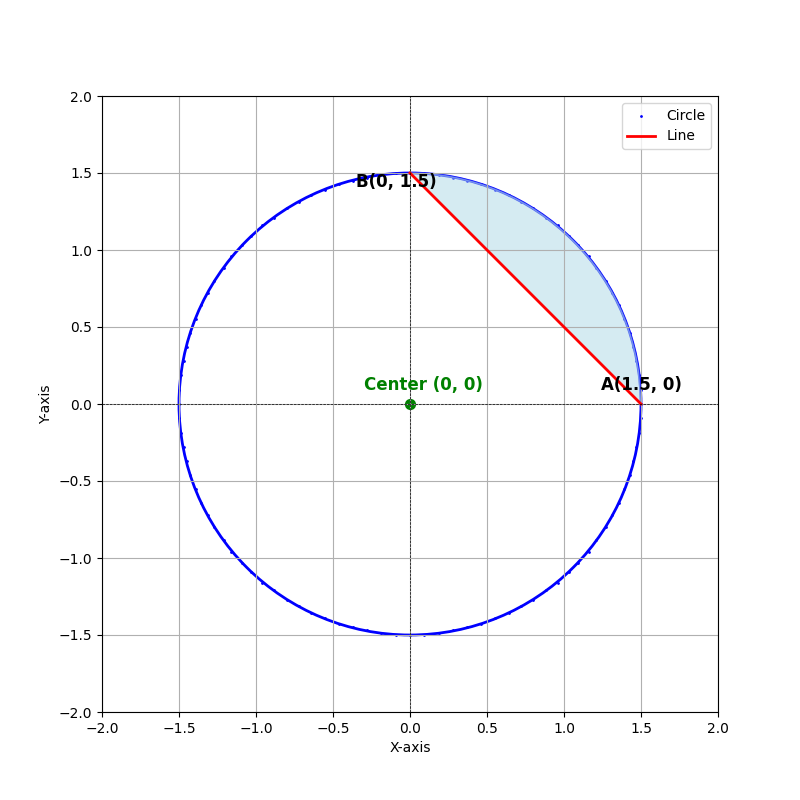
\includegraphics[width=0.7\linewidth]{figs/plot.png}
   \caption{ }
   \label{plot}
\end{figure}\\
The given circle can be expressed as conics with parameters,\\
\begin{align}
    V=\myvec{4 & 0\\0 & 4},u=0,f=-9.\\
\end{align}
The line parameters are:\\

\begin{align}
    h=\myvec{0\\ \frac{3}{2}},m=\myvec{1\\-1}.
\end{align}
The points of intersection of the line 
\begin{align}
L: \quad x = h + \kappa m \quad \kappa \in \mathbb{R}
\label{eq:conic_tangent}
\end{align}
with the conic section \begin{align}
	\text{g}\brak{x} = x^{\top}Vx+2u^{\top}x+f=0
    \end{align} are given by
\begin{align}
x_i = h + \kappa_im
	\label{eq:chord-pts}
\end{align}
where,
    \begin{multline}
\kappa_i = \frac{1}
{
m^{\top}Vm
}
\lbrak{-m^{\top}\brak{Vh+u}}
%\\
\pm
%{\small
\rbrak{\sqrt{
\sbrak{
m^{\top}\brak{Vh+u}
}^2
	-\text{g}
\brak
{h
%\vec{h}^{\top}\vec{V}\vec{h} + 2\vec{u}^{\top}\vec{h} +f
}
\brak{m^{\top}Vm}
}
}
%}
\label{eq:app-tangent_roots}
\end{multline}
Substituting the parameters in above Equation:\\
\begin{align}
    k=0,\frac{3}{2}.\\
\end{align}
yielding the points of intersection as:\\
\begin{align}
    A=\myvec{\frac{3}{2}\\0},B=\myvec{0\\ \frac{3}{2}}
\end{align}
From ,\figref{plot}the desired area is:\\
\begin{align}
\int_{0}^{\frac{3}{2}}\frac{\sqrt{9-4x^2}}{2}-\int_{0}^{\frac{3}{2}}\frac{3-2x}{2}=\frac{9}{16}\pi-\frac{9}{8}\\
\end{align}
\begin{table}[h]
    \centering
    \begin{tabular}{|c|c|}
        \hline
        Point & Coordinates\\
        \hline
        $A$ & \myvec{0\\6}\\
        \hline
        $B$ & \myvec{8\\0}\\
        \hline
        $C$ & \myvec{0\\0}\\
        \hline
\end{tabular}

    \caption{3.1}
    \label{}
\end{table}
\end{document}